%% 
%% Copyright 2019-2020 Elsevier Ltd
%% 
%% This file is part of the 'CAS Bundle'.
%% --------------------------------------
%% 
%% It may be distributed under the conditions of the LaTeX Project Public
%% License, either version 1.2 of this license or (at your option) any
%% later version.  The latest version of this license is in
%%    http://www.latex-project.org/lppl.txt
%% and version 1.2 or later is part of all distributions of LaTeX
%% version 1999/12/01 or later.
%% 
%% The list of all files belonging to the 'CAS Bundle' is
%% given in the file `manifest.txt'.
%% 
%% Template article for cas-dc documentclass for 
%% double column output.

%\documentclass[a4paper,fleqn,longmktitle]{cas-dc}
\documentclass[a4paper,fleqn]{cas-dc}

%\usepackage[authoryear,longnamesfirst]{natbib}
%\usepackage[authoryear]{natbib}
\usepackage[numbers]{natbib}

\begin{comment}
\def\tsc#1{\csdef{#1}{\textsc{\lowercase{#1}}\xspace}}
\tsc{WGM}
\tsc{QE}
\tsc{EP}
\tsc{PMS}
\tsc{BEC}
\tsc{DE}
%%%
\end{comment}
%%%Author definitions


\begin{document}
	\let\WriteBookmarks\relax
	\def\floatpagepagefraction{1}
	\def\textpagefraction{.001}
	\shorttitle{Survey of Multimedia Data in Manufacturing}
%	\shortauthors{Yunchao Wang et~al.}
	
	\title [mode = title]{Visualization and Visual Analysis of Multimedia Data in Manufacturing: A Survey}                      
	%\tnotemark[1,2]
	
	\begin{comment}
	\tnotetext[1]{This document is the results of the research
	project funded by the National Science Foundation.}
	
	\tnotetext[2]{The second title footnote which is a longer text matter
	to fill through the whole text width and overflow into
	another line in the footnotes area of the first page.}
	
	\end{comment}
	
	
%	\author{Yunchao Wang}
%	\author {Zihao Zhu}
%	\author{Lei Wang}
%	\author{Guodao Sun*}
%	\ead{godoor.sun@zjut.edu.cn}
%	\author{Ronghua Liang}
%	\address{College of Computer Science, Zhejiang University of Technology, Hangzhou, 310023}
	

%	\author{Guodao Sun{mycorrespondingauthor}}
%\cortext[mycorrespondingauthor]{Corresponding author}
	
	\begin{comment}
	\author[1,3]{CV Radhakrishnan}[type=editor,
	auid=000,bioid=1,
	prefix=Sir,
	role=Researcher,
	orcid=0000-0001-7511-2910]
	\cormark[1]
	\fnmark[1]
	\ead{cvr_1@tug.org.in}
	\ead[url]{www.cvr.cc, cvr@sayahna.org}
	
	\credit{Conceptualization of this study, Methodology, Software}
	
	\address[1]{Elsevier B.V., Radarweg 29, 1043 NX Amsterdam, The Netherlands}
	
	\cortext[cor1]{Corresponding author}
	
	\cortext[cor2]{Principal corresponding author}
	\fntext[fn1]{This is the first author footnote. but is common to third
	author as well.}
	\fntext[fn2]{Another author footnote, this is a very long footnote and
	it should be a really long footnote. But this footnote is not yet
	sufficiently long enough to make two lines of footnote text.}
	
	\nonumnote{This note has no numbers. In this work we demonstrate $a_b$
	the formation Y\_1 of a new type of polariton on the interface
	between a cuprous oxide slab and a polystyrene micro-sphere placed
	on the slab.
	}
	\end{comment}
	
	
	\begin{keywords}
		Visualization \sep Visual Analysis \sep Manufacturing \sep Multi-media data \sep Industry 4.0
	\end{keywords}
	
	
	\begin{abstract}
		%随着生产技术和社会需求的发展,制造业的门类不断完善。而传感器和计算机的使用,使得制造业中多媒体数据的收集越来越方便。根据多媒体数据的类型进行针对性的快速细致的分析可以在制造业全流程的不同阶段做出及时的决策。可视化与可视分析因其直观性和可交互性,在数据的理解、展示和分析上展现了强大的能力,被频繁应用在制造业多媒体数据分析中。在本文中,我们提出了一个可视化与可视分析的文献综述,专门为制造业多媒体数据。我们根据可视化技术、交互分析方法和应用领域对现有研究进行分类。在制造业研究项目的具体例子中,我们讨论了可视化和可视化分析应用于不同类型的多媒体数据时的差异。最后,我们对现有挑战做了总结,指出未来研究方向。
		With the development of production technology and social needs, sectors of manufacturing are constantly improving. The use of sensors and computers has made it increasingly convenient to collect multimedia data in manufacturing. Targeted, rapid and detailed analysis based on the type of multimedia data can make timely decisions at different stages of the entire manufacturing process. Visualization and visual analytics are frequently adopted in manufacturing multimedia data analysis because of their powerful ability to understand, present and analyze data in an intuitive and interactive way. In this paper, we present a literature review of visualization and visual analytics specifically for manufacturing multimedia data. We classify existing researches according to visualization techniques, interaction analysis methods and application areas. We discuss the differences when visualization and visual analytics are applied to different types of multimedia data in the context of specific examples from manufacturing research projects. Finally, we summarize the existing challenges and prospect the future research directions.
	\end{abstract}
	
	\maketitle
	
%工业4.0的核心是智能生产技术和智能生产模式,旨在通过“物联网”和“务联网”,把产品、机器、资源和人联系在一起,推动各环节数据共享,实现产品全生命周期和全制造流程的数字化。
%The core of Industry 4.0 is smart production technology and model. It aims to connect products, machines, resources and people through the \textit{Internet of Things} (IoT)~\cite{gubbi2013internet} and \textit{Internet of Services} (IoS)~\cite{cardoso2008service}, promote data sharing in all aspects, and realize the digitalization of the whole product life cycle and the whole manufacturing process.

%通过广泛的文献回顾,添加了最近出现的新方法,并按照新的角度对主题进行重新分类。
 


%  调查的范围
\section{Scope of the Survey}
%为了阐明本调查的范围,我们阐明了我们工作中使用的三个术语:制造业、多媒体数据和可视化/可视分析。
To clarify the scope of this survey, we articulate three terms used in our work: manufacturing, multimedia data, and visualization/visual analytics.
%首先要说明是制造业是我们调查的领域。
First, it is important to note that manufacturing is the area we investigated.
%随着生产技术和社会需求的发展,制造业的门类不断完善。
With the development of production technology and social demand, the categories of manufacturing industry have been improved.
%现在中国国民经济行业分类中,制造业有31个大类,179个中类,609个小类。
Nowadays, there are 31 major categories, 179 medium categories and 609 small categories in China's national economic industry classification.
%我们主要对其中计算机技术普及程度较高的制造业类别进行调查。
We focus on those manufacturing categories which have a high degree of computer technology and automation.
%例如计算机制造、汽车整车制造、家用电力器具制造等。
For example, computer manufacturing, automobile manufacturing, household electric appliance manufacturing, etc.
%其次我们的分析对象是制造业全流程的多媒体数据,包括了结构化数据和非结构化数据。
Secondly, we analyze multimedia data from the whole process of manufacturing industry, including both structured and unstructured data. 
%传感器和计算机的使用,使得制造业中多媒体数据的收集越来越方便。
The usage of sensors and computers has made it increasingly convenient to collect multimedia data in manufacturing.
%因此,数据自身的实时性和数据间的关联性也有所增强。
Consequently, the real-time nature of data itself and the correlation between data have been enhanced.
%多媒体数据可以大致分为:表格文本数据,传感信号数据、音频数据、图像数据和视频数据。
Multimedia data can be broadly classified into: ``tabular text data", ``signal sensing data", ``audio data", ``image data" and ``video data".
%根据多媒体数据的类型进行针对性的快速细致的分析可以在制造业全流程的不同阶段做出及时的决策。
Targeted, rapid and detailed analysis based on the type of multimedia data can make timely decisions at different stages of the entire manufacturing process.
%这也是对制造业多媒体数据进行研究的内驱动力。
It is also the internal motivation for research on multimedia data in manufacturing.
%最后,我们我们关注的是运用在这些研究中的可视化与可视分析技术。
Finally, we are concerned with the visualization and visual analytics techniques used in these studies.
%可视化/可视分析技术因其直观性和有效性,被频繁应用在制造业多媒体数据的分析中。
Visualization/visual analysis techniques are frequently used in the analysis of multimedia data in the manufacturing industry because of their intuitiveness and effectiveness.
%我们希望调查在制造业多媒体数据分析中的可视化/可视分析技术,发现可视化研究社区感兴趣的应用领域,以及具体使用的可视化技术和交互分析方法。
We attempt to investigate visualization and visual analytics techniques of multimedia data in manufacturing to discover application areas of interest to the visualization research community, as well as visualization techniques and interactive analysis methods.

%我们对在可视化会议或者期刊上已发表的论文进行了关键词搜索。
We conducted a keyword search for papers that have been published in visualization conferences or journals to collect suitable literature.
%关键词的例子包括但不限于“制造业”,“工业”,“智能制造”,“制造业流程”,“工业4.0”。
Examples of keywords include but are not limited to "manufacturing", "industrial", "smart manufacturing", "manufacturing process ", "Industry 4.0".
%此外,我们的工作试图在其他高质量综述的基础上,探索制造业中可视化研究社区感兴趣的可视化技术、交互分析方法和应用领域。
Moreover, our work attempts to explore visualization techniques, interactive analysis methods, and application areas of interest to the visualization research community in manufacturing, building on other high-quality reviews~\cite{shi2020visual, wang2018visualization}.

% 相关调查
\section{Related Surveys}
%因为制造业门类繁多,流程复杂,针对制造业的工作的研究方向和研究对象很多。
Because the manufacturing industry has a wide range of categories and complex processes, there are many research directions and research objects for the manufacturing industry.
%有一部分调查是从微观的视角出发,对制造业中的具体技术或数据的相关工作进行总结。
One part of the survey is a summary of the work related to specific technical or data in manufacturing from a micro perspective~\cite{bruno2006visualization, stevens2007visualization, berg2017industry}. 
%Bruno等介绍了增强现实中的工业工程数据可视化的应用。
Bruno et al.~\cite{bruno2006visualization} presented the application of industrial engineering data visualization in augmented reality.
%Stevens等针对复杂汽车数据可视化做了总结,讨论了可视化在汽车制造中的作用。
Stevens et al.~\cite{stevens2007visualization} summarized    for complex automotive data visualization and discuss the role of visualization in automotive manufacturing.
%berg等仅仅对虚拟现实在产品设计和制造中的工业应用做了调查。
Berg et al.~\cite{berg2017industry} merely investigated the industrial applications of virtual reality in product design and manufacturing.
%另一部分调查是从宏观的视角出发,对整个制造业中的数据,技术或者应用的相关工作进行总结。
Another part of the survey is a summary of the work related to data, techniques or application areas in the entire manufacturing industry from a macro perspective~\cite{yin2014review, liu2021survey, zhou2019survey, font2019interactive, de2020survey}.
%Yin等人围绕工业过程监测的基本数据驱动方法做了细致的调查
Yin et al.~\cite{yin2014review} made a detailed investigation around the basic data-driven approach to industrial process monitoring
%Liu等人根据生产过程收集并统计了常见的制造业数据类型,并按照数据属性进行归纳总结。他们还介绍了可视化时间、空间、时空结合的数据时常用的形式。
Liu et al.~\cite{liu2021survey} collected and counted common manufacturing data types based on production processes and summarized them by data attributes. They also introduced the common forms used when visualizing temporal, spatial, and spatio-temporal combined data.
%Zhou等人对可视化在智能制造中的应用做了专门的调查。其从应用场景和行业领域对现有研究进行分类。
Zhou et al.~\cite{zhou2019survey} provided a specifically tailored survey on visualization in smart manufacturing. It classifies existing research in terms of application areas and industry sectors.
%David等人通过实例,探讨了交互式可视化的价值,并强调了工业工程社区在交互式可视化过程中必须面对的挑战,包括技术和知识限制、用户交互限制以及实现策略。 
Using examples, David et al.~\cite{font2019interactive} explored the value of interactive visualization and highlighted the challenges that industrial engineering community must face in the interactive visualization process, including technical and knowledge limitations, user interaction limitations, and implementation strategies. 
%Cardoso等人通过系统的文献综述评估增强现实的适用性和适用性对真实工业过程的影响,主要包括增强现实技术是如何应用的,哪些行业对该技术最感兴趣,该技术是如歌发展以满足行业需求的,以及增强现实的好处和挑战。
Cardoso et al.~\cite{de2020survey} assessed the applicability and applicability of augmented reality to real industrial processes through a systematic literature review that focuses on how augmented reality is being applied, which industries are most interested in the technology, how the technology is evolving to meet industry needs, and the benefits and challenges of augmented reality.    

\begin{figure}[t]
	\centering
	\vspace{.5em}
	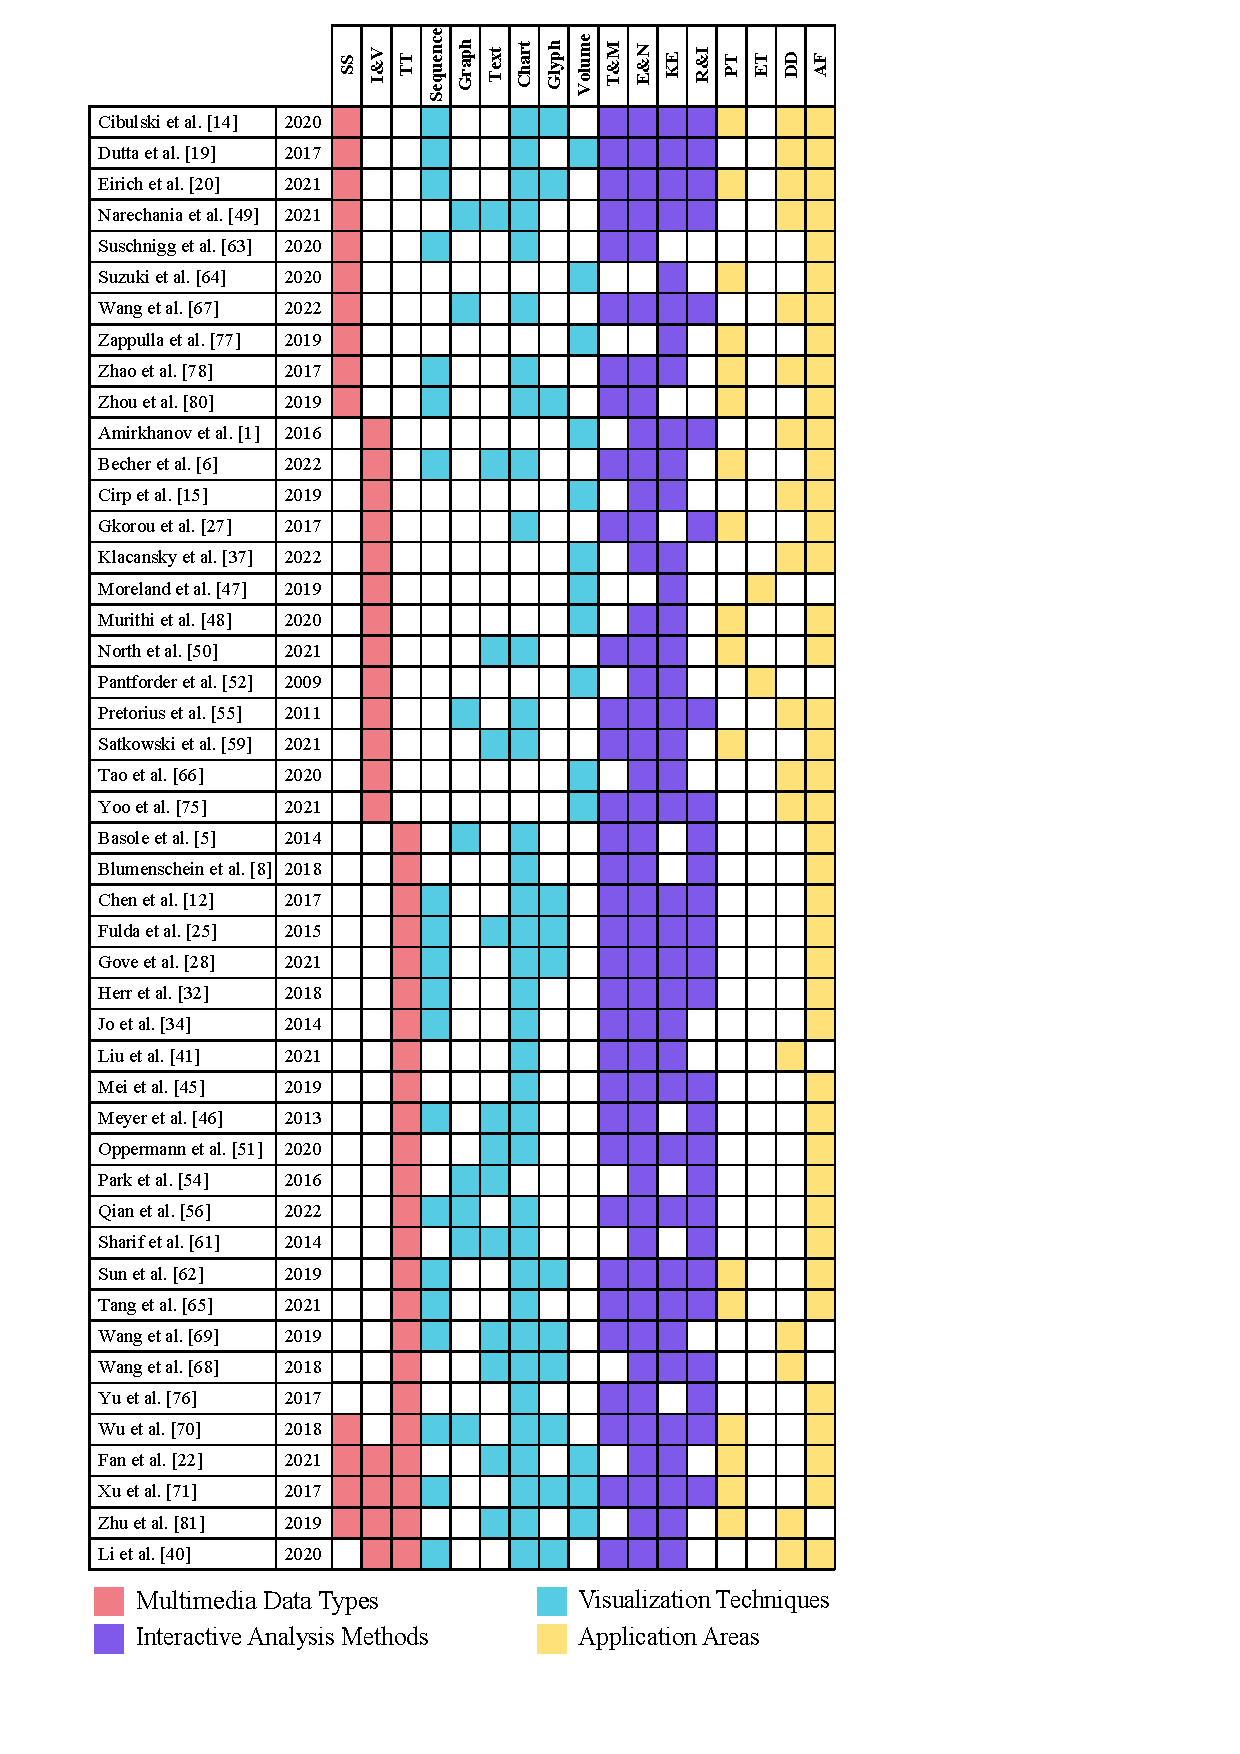
\includegraphics[width=0.48\textwidth]{Images/table.pdf}
	\caption{Categorization of the literature published in each section of this paper is based on manufacturing multimedia data types, visualization techniques, interaction analysis methods, and application areas.}
	\vspace{-1em}
	\label{fig:Classification_Coordinate}
\end{figure}

% 分类法
\section{Taxonomy}
%受上述高质量综述的启发,我们提出了一种新的基于数据类型的分类方法,对制造业多媒体数据的可视化与可视分析进行总结。
Inspired by the above high-quality reviews, we propose a novel data type-based classification method to summarize the visualization and visual analysis of multimedia data in manufacturing. 
%我们添加了最近发表的工作,并从可视化技术、交互式分析方法和应用领域进行详细讨论。
We add recently published works and discuss them in detail in terms of visualization techniques, interactive analysis methods and application areas.
%图1所示为我们的文献分类。纵轴为基于制造业多媒体数据的论文。纵轴为具体类别(红色为多媒体数据类型、蓝色为可视化技术、紫色为交互式分析方法、黄色为应用)。
Fig~\ref{fig:Classification_Coordinate} shows the classification of the literature. The vertical axis shows papers based on multimedia data in manufacturing. The horizontal axis shows specific categories (
\raisebox{-0.4mm}{
\includegraphics[scale=0.25]{Images/red.png}} for multimedia data types, 
\raisebox{-0.4mm}{
\includegraphics[scale=0.25]{Images/blue.png}} for visualization techniques, 
\raisebox{-0.4mm}{
\includegraphics[scale=0.25]{Images/purple.png}} for interactive analysis methods, and 
\raisebox{-0.4mm}{
\includegraphics[scale=0.25]{Images/yellow.png}} for application areas).

%多媒体数据类型。
\raisebox{-0.4mm}{
\includegraphics[scale=0.25]{Images/red.png}} \textbf{Multimedia data types}. 
%我们将多媒体数据按照数据类型分为:表格文本数据、传感信号数据和图像视频数据。
We categorize multimedia data according to data types: \textit{Tabular text data} (TT), \textit{Signal sensing data} (SS), and \textit{Image \& video data} (I\&V). 

%可视化技术。
\raisebox{-0.4mm}{
\includegraphics[scale=0.25]{Images/blue.png}} \textbf{Visualization techniques}.
%我们将可视化技术分为序列可视化、图形可视化、文本可视化、图表可视化、符号可视化和体可视化。
We categorize visualization techniques into \textit{Sequence}, \textit{Graph}, \textit{Text}, \textit{Chart}, \textit{Glyph}, and \textit{Volume} visualizations.

%交互式分析方法。
\raisebox{-0.4mm}{
\includegraphics[scale=0.25]{Images/purple.png}} \textbf{Interactive analysis methods}.
%可视化系统中的交互分析方法分为追踪监控、探索导航、知识外化、模式识别和细化识别。
Interaction analysis methods in visualization systems are classified into \textit{Tracking \& Monitoring} (T\&M), \textit{Exploration \& Navigation} (E\&N), \textit{Knowledge Externalization} (KE), \textit{Pattern Discovery} (PD), and \textit{Refinement \& Identification} (R\&I). 

%应用。
\raisebox{-0.4mm}{
\includegraphics[scale=0.25]{Images/yellow.png}} \textbf{Application areas}.
%应用领域可以分为设计研发、工业生产、教育培训和分析反馈。
The application areas categorized into \textit{Design \& Development} (DD), \textit{Industrial Production} (IP), \textit{Education \& Training} (ET), and \textit{Analytical \& Feedback} (AF), depending on phases and functions.

%这幅图中可以发现以下几个模式。
The following patterns can be found in Fig~\ref{fig:Classification_Coordinate}.
%首先可视化技术中的“volume”,常用在I&V数据类型中,而“chart”和“Sequence”在“TT”和“S”数据类型中应用的较多。
First of all, the visualization technique \textit{Volume} is commonly used in I\&V, while \textit{Chart} and \textit{Sequence} are more often used in TT and S. 
%其次可视化系统的文章通常具备三种以上的交互式分析方法,其中最多使用的是“E\&N”、“PD”和“R\&I”
Secondly, articles of visualization systems usually have more than three interactive analysis methods, among which the most used are E\&N, PD and R\&I.

\bibliographystyle{cas-model2-names}
\bibliography{SISI_dc}

\end{document}

